\chapter{Rancangan Sistem}
\label{app:rancangan}

Arsitektur sistem \emph{chatbot} hukum yang dikembangkan terdiri atas sejumlah komponen yang saling terhubung dan bekerja secara terintegrasi dalam satu \emph{workflow} pemrosesan \emph{end-to-end}. Setiap komponen berada dalam cakupan satu atau lebih modul utama sistem, yaitu Modul data \emph{ingestion} (\emph{scraping} dan \emph{parsing}) serta modul \emph{admin} dan \emph{landing page}, Modul \emph{Document Processing Orchestrator} (DPO) dan \emph{query pre-planning}, Lapisan \emph{Explainable AI} (XAI) serta modul \emph{chat}, dan Modul \emph{hybrid retrieval} dan \emph{Knowledge Graph} serta modul autentikasi. Berikut diagram arsitektur dari sistem hukum, sebagaimana ditunjukkan pada Gambar~\ref{fig:architecture-dpo} dan Gambar~\ref{fig:architecture-rag}.

\begin{figure}[H]
    \centering
    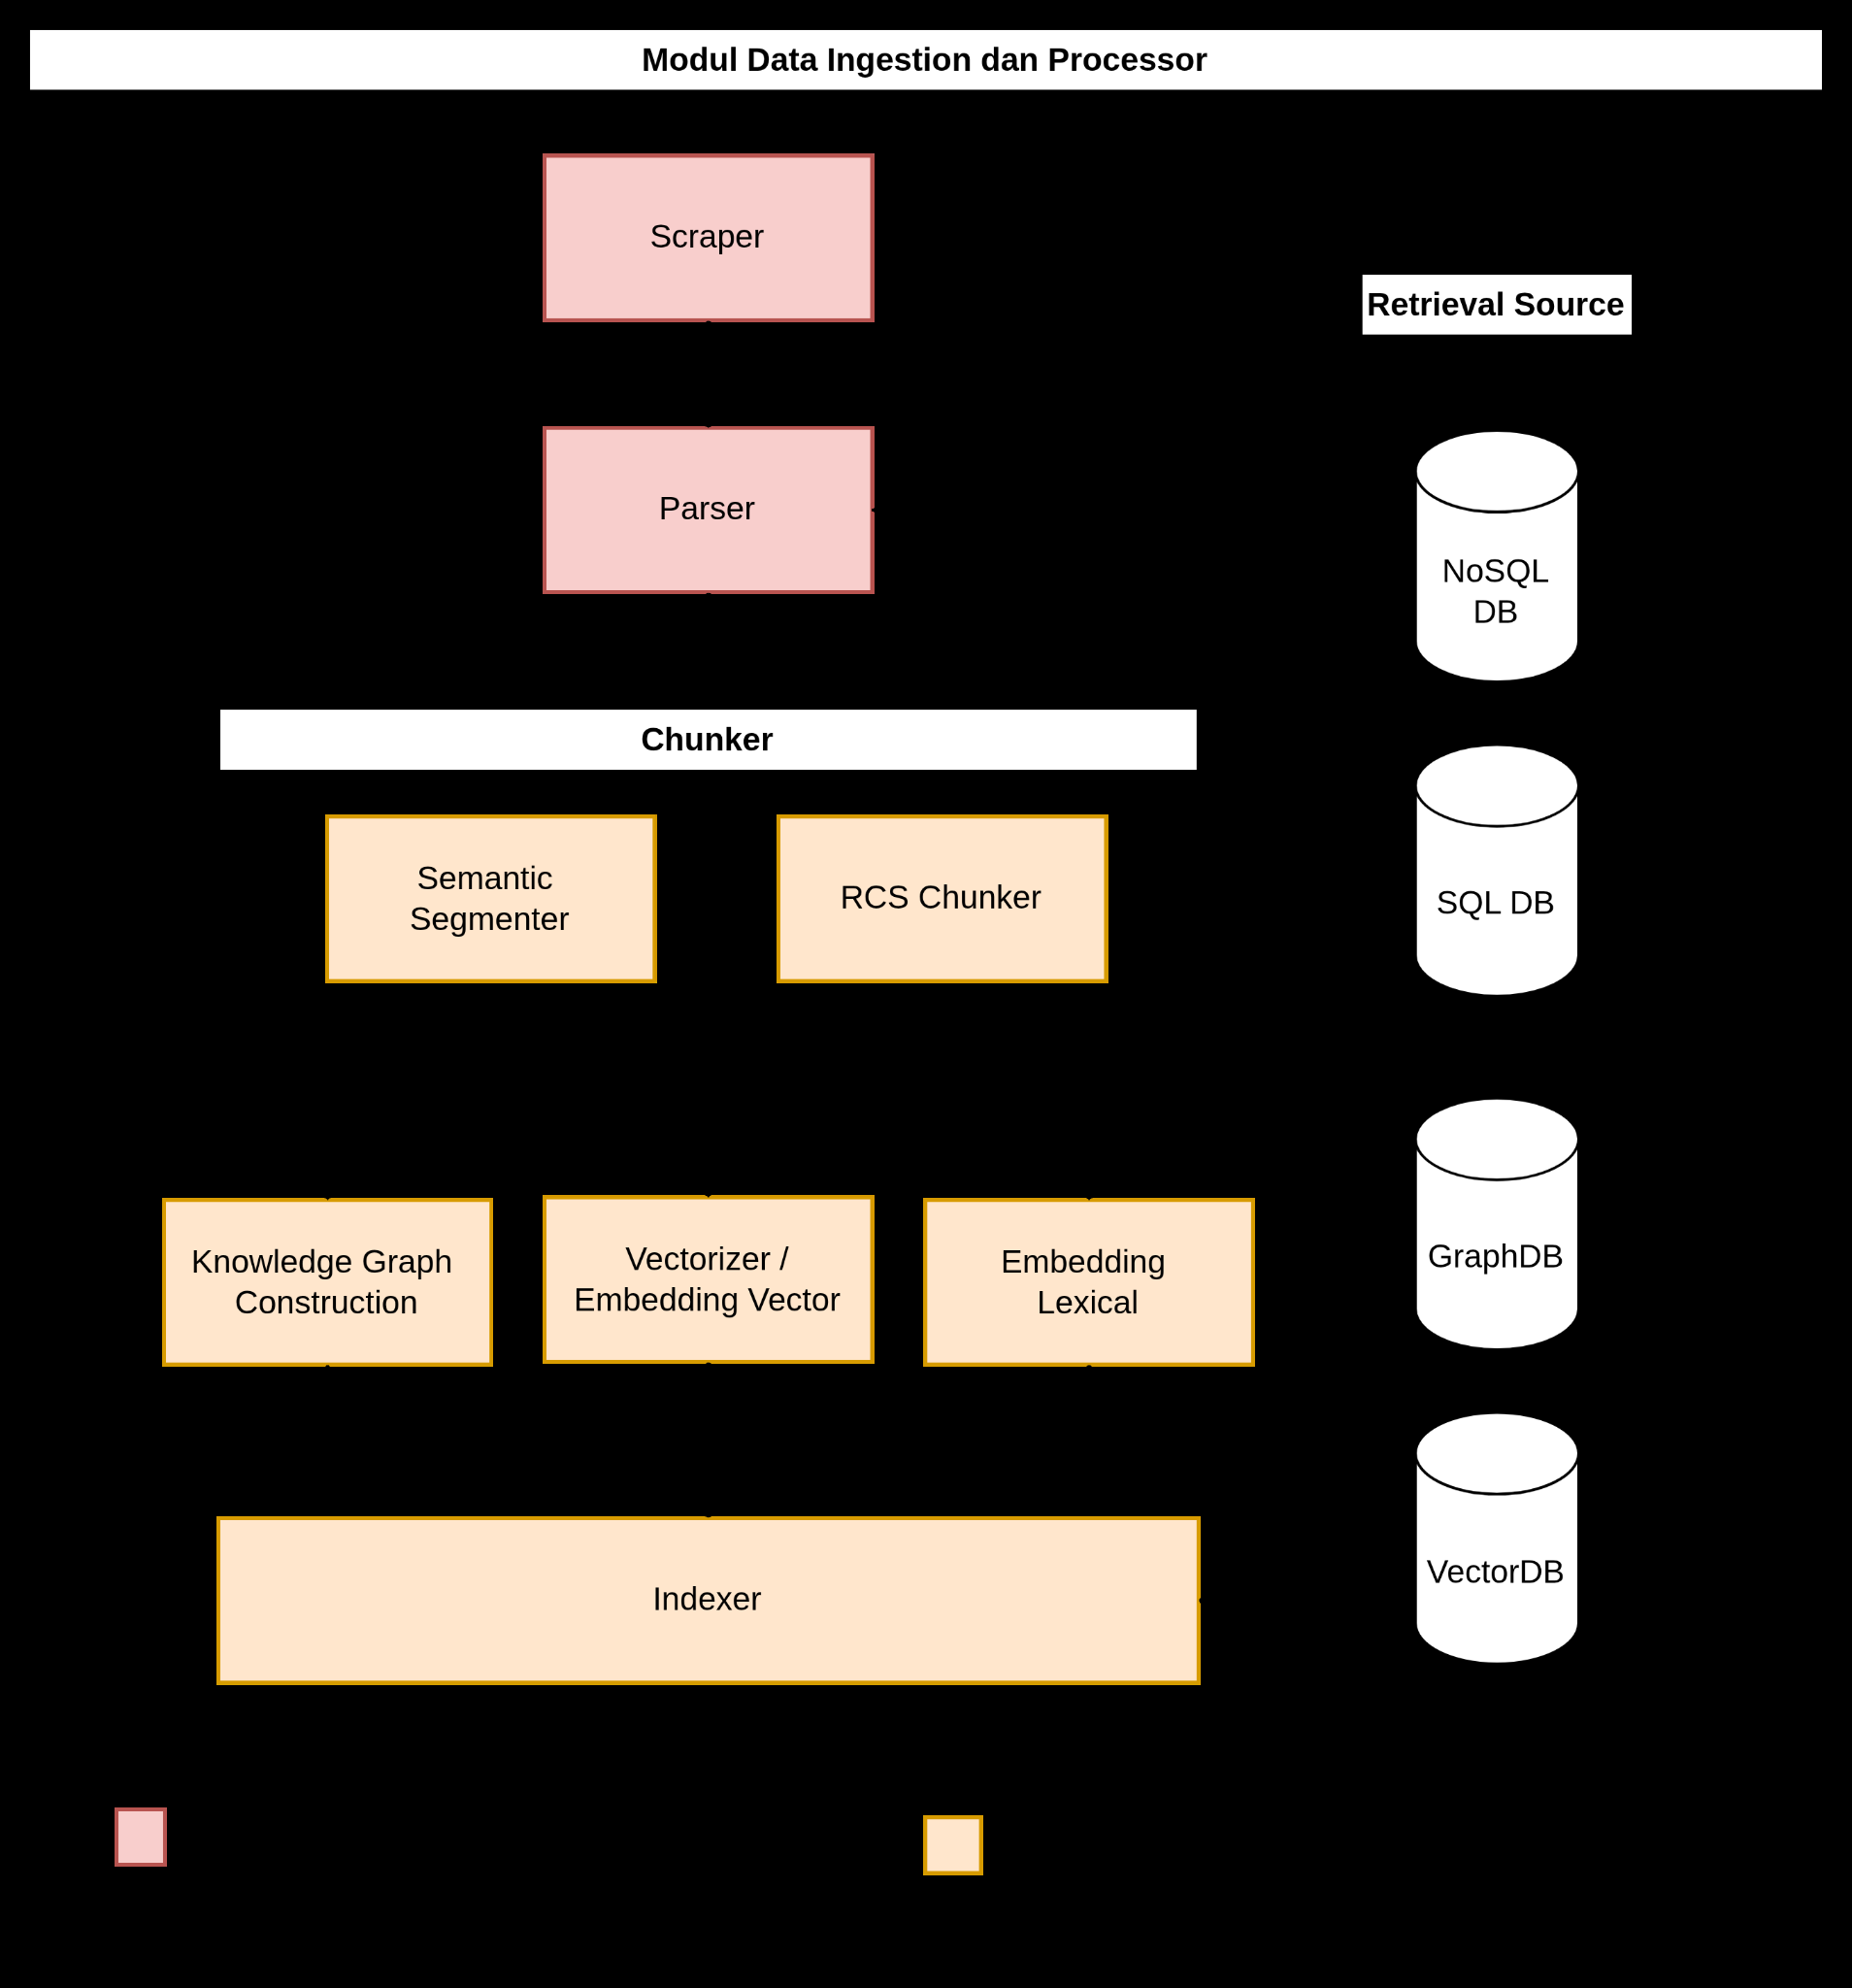
\includegraphics[width=0.78\textwidth]{images/reference-015.png}
    \caption{Diagram Arsitektur Sistem \emph{Chatbot} Hukum bagian DPO.}
    \label{fig:architecture-dpo}
\end{figure}

\begin{figure}[H]
    \centering
    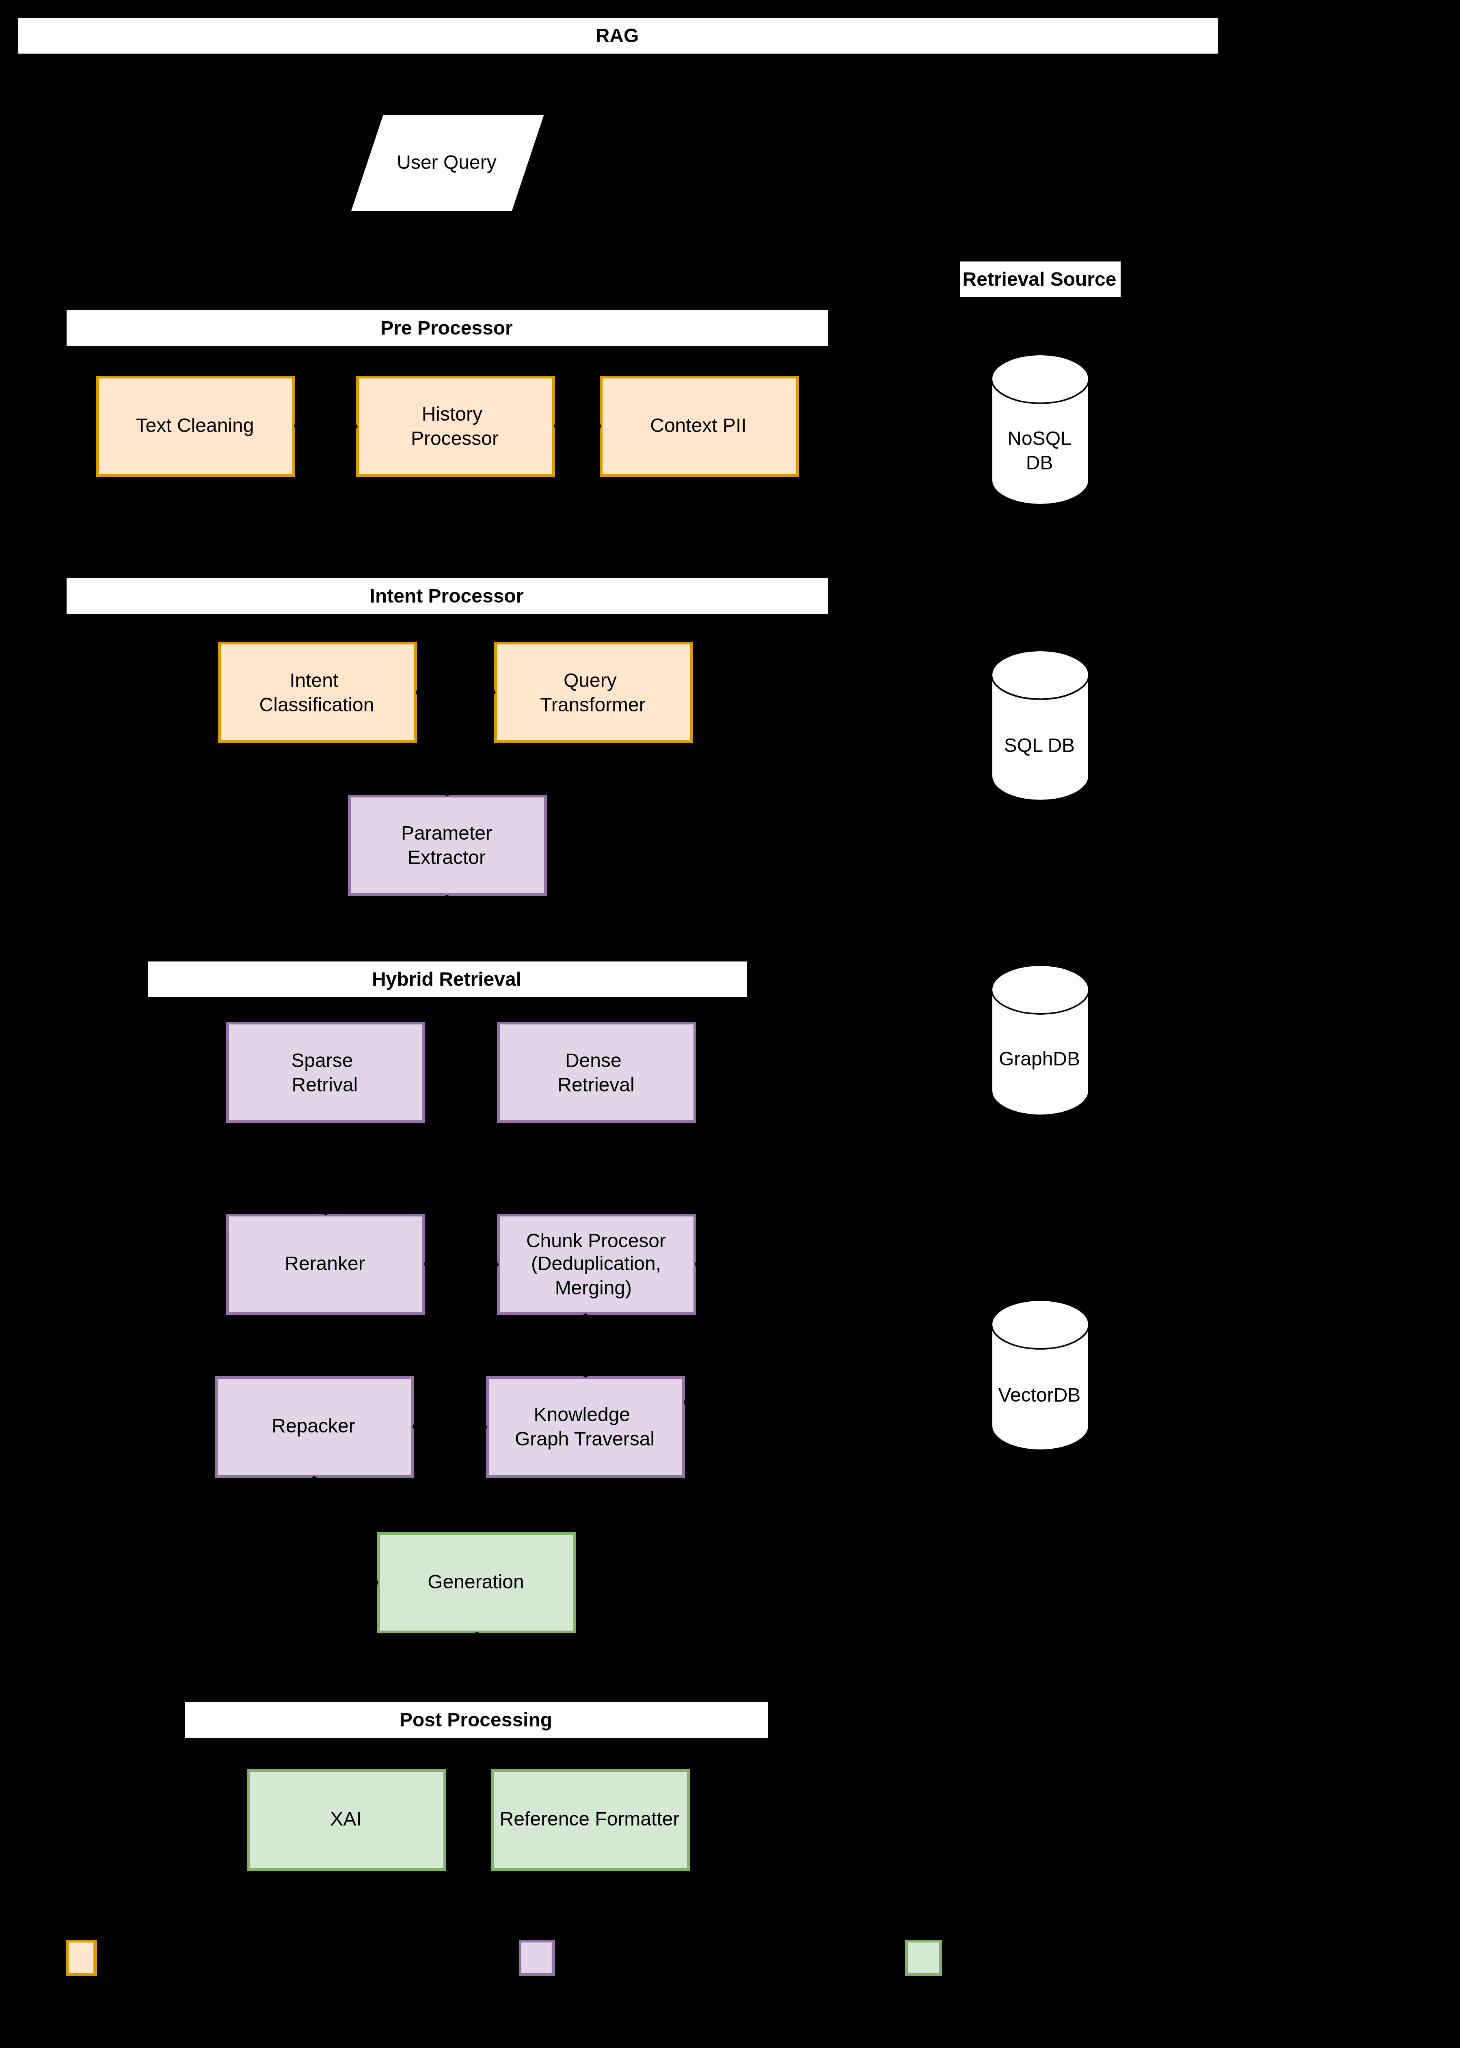
\includegraphics[width=0.58\textwidth]{images/reference-017.png}
    \caption{Diagram Arsitektur Sistem \emph{Chatbot} Hukum bagian RAG.}
    \label{fig:architecture-rag}
\end{figure}

Berikut merupakan penjelasan dari masing-masing komponen yang akan dikembangkan. Komponen DPO dan RAG dirangkum pada Tabel~\ref{tab:dpo-components} dan Tabel~\ref{tab:rag-components}.

\begin{table}[H]
\centering
\caption{Deskripsi Komponen \emph{Data Processing Orchestrator} (DPO)}
\label{tab:dpo-components}
\small
\begin{tabularx}{\textwidth}{|p{0.27\textwidth}|X|}
\hline \textbf{Komponen} & \textbf{Deskripsi} \\\hline
\emph{Scraper} & Komponen yang bertugas mengambil dokumen peraturan perundang-undangan dari sumber resmi secara otomatis. \\\hline
\emph{Parser} & Komponen yang mem-\emph{parsing} dokumen hukum ke dalam struktur hierarkis antara lain undang-undang, bab, bagian, pasal, dan ayat. \\\hline
\emph{Chunker} & Komponen yang melakukan segmentasi dokumen hukum menjadi unit lebih kecil menggunakan \emph{Semantic Segmenter} dan \emph{RCS Chunker}. \\\hline
\emph{Knowledge Graph Construction} & Komponen yang membangun \emph{Knowledge Graph} berdasarkan relasi antara peraturan dan pasal yang teridentifikasi. \\\hline
\emph{Vectorizer (Embedding Vector)} & Komponen yang membentuk representasi \emph{embedding vector} dari \emph{chunk} dokumen hukum untuk mendukung metode \emph{dense retrieval}. \\\hline
\emph{Embedding Lexical} & Komponen yang membentuk \emph{embedding} berbasis leksikal untuk mendukung metode \emph{sparse retrieval}. \\\hline
\emph{Indexer} & Komponen yang mengindeks hasil pemrosesan data ke dalam basis data vektor agar dapat digunakan secara efisien pada tahap \emph{retrieval}. \\\hline
\end{tabularx}
\end{table}

\begin{table}[H]
\centering
\caption{Deskripsi Komponen \emph{Retrieval-Augmented Generation} (RAG)}
\label{tab:rag-components}
\footnotesize
\begin{tabularx}{\textwidth}{|p{0.27\textwidth}|X|}
\hline \textbf{Komponen} & \textbf{Deskripsi} \\\hline
\emph{Pre Processor} & Tahap awal pemrosesan \emph{query} yang mencakup \emph{text cleaning}, pemrosesan riwayat percakapan, serta pengelolaan konteks informasi sensitif sebelum \emph{query} diproses lebih lanjut. \\\hline
\emph{Intent Processor} & Komponen yang melakukan klasifikasi \emph{intent} \emph{query} pengguna dan mentransformasikan \emph{query} agar selaras dengan struktur serta terminologi hukum formal. \\\hline
\emph{Parameter Extractor} & Komponen yang mengekstraksi parameter penting dari \emph{query}, seperti jenis peraturan, nomor undang-undang, pasal, ayat, dan entitas hukum relevan lainnya. \\\hline
\emph{Hybrid Retrieval} & Komponen yang melakukan pencarian konteks hukum secara paralel menggunakan metode \emph{sparse retrieval} dan \emph{dense retrieval} untuk memperoleh hasil yang relevan. \\\hline
\emph{Reranker} & Komponen yang mengurutkan ulang hasil \emph{retrieval} berdasarkan tingkat relevansi terhadap \emph{query} pengguna. \\\hline
\emph{Chunk Processor} & Komponen yang melakukan deduplikasi dan penggabungan \emph{chunk} hasil \emph{retrieval} untuk menghilangkan redundansi dan membentuk konteks yang lebih baik. \\\hline
\emph{Knowledge Graph Traversal} & Komponen yang menelusuri relasi antara peraturan dan pasal pada \emph{Knowledge Graph} untuk memperluas konteks hukum yang relevan. \\\hline
\emph{Repacker} & Komponen yang menyusun ulang konteks hukum hasil \emph{retrieval} dan \emph{traversal} ke dalam format terstruktur yang siap digunakan pada tahap \emph{generation}. \\\hline
\emph{Generation} & Tahap yang menghasilkan jawaban hukum berdasarkan konteks akhir yang telah disusun oleh sistem. \\\hline
\emph{Post Processing} & Tahap akhir pemrosesan yang mencakup perapihan jawaban, penyusunan sitasi hukum, serta integrasi mekanisme \emph{explainability}. \\\hline
\emph{Explainable AI (XAI)} & Komponen yang menyediakan penjelasan terhadap jawaban sistem, seperti \emph{input saliency}, \emph{source attribution}, dan visualisasi jalur \emph{reasoning}. \\\hline
\emph{Reference Formatter} & Komponen yang memformat referensi hukum agar tersaji secara konsisten dan mudah ditelusuri oleh pengguna. \\\hline
\end{tabularx}
\end{table}
